\documentclass[aspectratio=169]{beamer}
\usepackage{multimedia}
% Load Packages
\usepackage[utf8]{inputenc}
\usepackage{xcolor}
\usepackage{tikz} 
\usetikzlibrary{positioning,calc}
\usepackage{graphicx}
\usepackage{hyperref}
\usepackage{amsmath}
\usepackage{listings}
\usepackage{fontawesome}
\usepackage[center]{caption}
\usepackage{makecell}
\usepackage{adjustbox}
\usepackage{multirow}
\usepackage{multicol}
\usepackage{xspace} 
\usepackage{etoolbox} % for text size in table
\usepackage{booktabs} % for \midrule and other
\usepackage{pgfgantt} % for Gentt Chart


% Define Commands
\newcommand*{\ClipSep}{0.06cm} %To adjust footer logo
\newcommand{\E}{\mathrm{e}\,} %\def\I{e} % used to defined e for exp(x), see later what it should be
\newcommand{\ud}{\mathrm{d}}
\lstset{numbers=left, numberstyle=\tiny, stepnumber=1,firstnumber=1,breaklines=true,
    numbersep=5pt,language=Python,
    stringstyle=\ttfamily,
    basicstyle=\footnotesize, 
    showstringspaces=false
}

% Remove table's caption using the caption package
\captionsetup{labelformat=empty}

% For smaller size bibliography at the end slide
\setbeamerfont{bibliography entry author}{shape=\scshape,size=\tiny}%
\setbeamerfont{bibliography entry title}{shape=\scshape,size=\tiny}
\setbeamerfont{bibliography entry journal}{shape=\scshape,size=\tiny}
\setbeamerfont{bibliography entry note}{shape=\scshape,size=\tiny}

% Numbered items in Bibliography
\setbeamertemplate{bibliography item}{\insertbiblabel}

% -------------------------------------------
% Defining TikZ geometrics 
% -------------------------------------------

% Tikz library
\usepackage{tikz}
\usetikzlibrary{shapes.geometric, arrows}

% Defining Tickz Style
\tikzstyle{startstop} = [rectangle, rounded corners, minimum width=3cm, minimum height=1cm, text centered, draw=black, fill=red!40]

\tikzstyle{startstop1} = [rectangle, rounded corners, minimum width=3cm, minimum height=1cm, text centered, draw=black, fill=pink!30]

\tikzstyle{startstop2} = [rectangle, rounded corners, minimum width=3cm, minimum height=1cm, text centered, draw=black, fill=teal!10]

\tikzstyle{io} = [trapezium, trapezium left angle=70, trapezium right angle=110, minimum width=3cm, minimum height=1cm, text centered, text width = 4.5cm, draw=black, fill=blue!30]

\tikzstyle{process} = [rectangle, minimum width=3cm, minimum height=1cm, text centered, text width = 6cm, draw=black, fill=orange!30]

\tikzstyle{decision} = [diamond, minimum width=3cm, minimum height=1cm, text centered, draw=black, fill=green!30]

\tikzstyle{arrow} = [thick,->,>=stealth]





\usetheme{oxonian}

% Title page
\title{\textbf{\textcolor{purple}{DSO : Direct Sparse Odometry}}}


% Sub-title
\subtitle{Presentation}

\author{\footnotesize \textbf{\textcolor{blue}{\Large Udit Singh Parihar}} }


\date{} %\today

\begin{document}

{\setbeamertemplate{footline}{} 
\frame{\titlepage}}

%%%%%%%%%%%%%%%%%%%%%%%%%%%%%%%%%%%%%%%%
% Outline
\section*{Outline}
\begin{frame}
		{\textcolor{blue}{\textbf{Presentation Outline}}}\tableofcontents
\end{frame}

%%%%%%%%%%%%%%%%%%%%%%%%%%%%%%%%%%%%%%%%
% Section: Introduction 
%%%%%%%%%%%%%%%%%%%%%%%%%%%%%%%%%%%%%%%%
\section{\textbf{\textcolor{purple}{Introduction}}}
		\begin{frame}[plain]
				\vfill
			\centering
			\begin{beamercolorbox}[sep=8pt,center,shadow=true,rounded=true]{title}
				\usebeamerfont{title}\insertsectionhead\par%
				\color{oxfordblue}\noindent\rule{10cm}{1pt}
			\end{beamercolorbox}
			\vfill

			$$
				\mathbf{X}^*:=\underset{\mathbf{X}}{\operatorname{argmax}} P(\mathbf{Y} \mid \mathbf{X})
			$$
		$Y$ noisy measurements are use to caluculate unknown $X$ which is 3D world and camera pose.
	\end{frame}


%---------------------------------------
% Slide: Direct Vs Indirect Odometry
%---------------------------------------
\begin{frame}{\textcolor{blue}{\textbf{Direct Vs Indirect Methods}}}
	\vspace{-0.5cm}

	
	\begin{block}{\textbf{\textcolor{teal}{Indirect Methods}}}
	\begin{itemize}
			\item Keypoints and descriptors extraction and correspondences Matching
			\item Geometry and Camera motion is estimated using triangulation and Fundamental matrix decomposition
			\item Reprojection error minimization, using depth, camera matrix and pose
			\begin{equation}
				E = \sum_{i} \left|u_i - P X_i\right|^2
			\end{equation}
		\end{itemize}
	

	\end{block}

\end{frame}

%---------------------------------------
% Slide: Direct Vs Indirect Odometry 2
%---------------------------------------
\begin{frame}{\textcolor{blue}{\textbf{Direct Vs Indirect Methods}}}
	\vspace{-0.5cm}

	
	\begin{block}{\textbf{\textcolor{teal}{Direct Methods}}}
	\begin{itemize}
			\item Combines the correspondences matching and tracking into single step
			\item Use actual sensor values to estimate the camera pose and 3D world
			\item Minimizes the Photometric error
			\begin{equation}
				r_i(\xi):=\left(I_2\left(w\left(\mathbf{x}_i, d_i, \xi\right)\right)-I_1\left(\mathbf{x}_i\right)\right)^2
			\end{equation}
	\end{itemize}
	

	\end{block}

\end{frame}

%---------------------------------------
% Slide: Dense Vs Sparse
%---------------------------------------
\begin{frame}{\textcolor{blue}{\textbf{Sparse vs Dense}}}
	\vspace{-0.5cm}
	\begin{block}{\textbf{\textcolor{teal}{Sparse}}}
	\begin{itemize}
			\item Selected set of independent pixels are used
			\item Favours corners and edges in the image, with high intensity gradients
	\end{itemize}
	\end{block}

	\begin{block}{\textbf{\textcolor{teal}{Dense}}}
		\begin{itemize}
				\item Use all the pixels or connected subset of pixels 
				\item Incorporates the connectedness prior to favour smoothness
	\end{itemize}
	\end{block}

	% Image from pics/dense_sparse.png of width 0.8\textwidth and height 0.8\textheight
	\begin{figure}
		\centering
		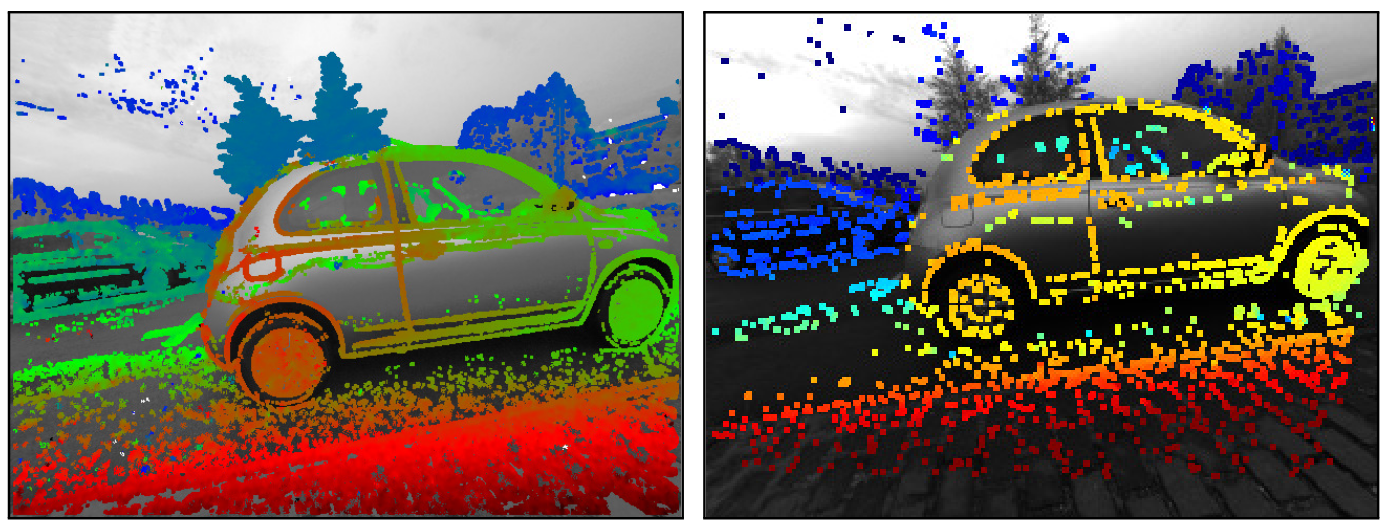
\includegraphics[height=0.2\textheight]{pics/dense_sparse.png}
		\caption{\scriptsize Dense LSD SLAM vs Sparse DSO}
	\end{figure}

\end{frame}


%--------------------------------------
% Slide: Filtering Vs Optimization
%--------------------------------------
\begin{frame}{\textcolor{blue}{\textbf{Filtering Vs Optimization}}}
	\vspace{-0.5cm}

	
	\begin{block}{\textbf{\textcolor{teal}{Filtering}}}
	\begin{itemize}
			\item Estimates and update the joint probability distribution over parameters using Kalman Filter
			\item Prediction step increases uncertainty while measurement reduces it
			\begin{equation}
				P\left(x_t, M \mid U_{t-1}, Z_t\right)
			\end{equation}
	\end{itemize}  
	\end{block}

	\begin{block}{\textbf{\textcolor{teal}{Optimization}}}
		\begin{itemize}
				\item Minimizes non-linear energy function using Gauss Newton
				\item Optimizes over keyframes for computational efficiency
				\begin{equation}
					P\left(X_t, M \mid U_{t-1}, Z_t\right)
				\end{equation}
		\end{itemize}
	\end{block}

\end{frame}

%%%%%%%%%%%%%%%%%%%%%%%%%%%%%%%%%%%%%%%%
% Section: Prior Work : LSD SLAM 
%%%%%%%%%%%%%%%%%%%%%%%%%%%%%%%%%%%%%%%%
\section{\textbf{\textcolor{purple}{Prior Art : LSD SLAM}}}
		\begin{frame}[plain]
				\vfill
			\centering
			\begin{beamercolorbox}[sep=8pt,center,shadow=true,rounded=true]{title}
				\usebeamerfont{title}\insertsectionhead\par%
				\color{oxfordblue}\noindent\rule{10cm}{1pt}
			\end{beamercolorbox}
			\vfill

	\end{frame}


%---------------------------------------
% Slide: Introduction
%---------------------------------------
\begin{frame}{\textcolor{blue}{\textbf{Introduction}}}
	\vspace{-0.5cm}
	\begin{block}{}
	\begin{itemize}
			\item Direct Monocular SLAM with scale-drift aware formulation including loop closures 
			\item Large scale consistent maps with high accuracy on CPU
	\end{itemize}
	\end{block}

	\begin{figure}
		\centering
		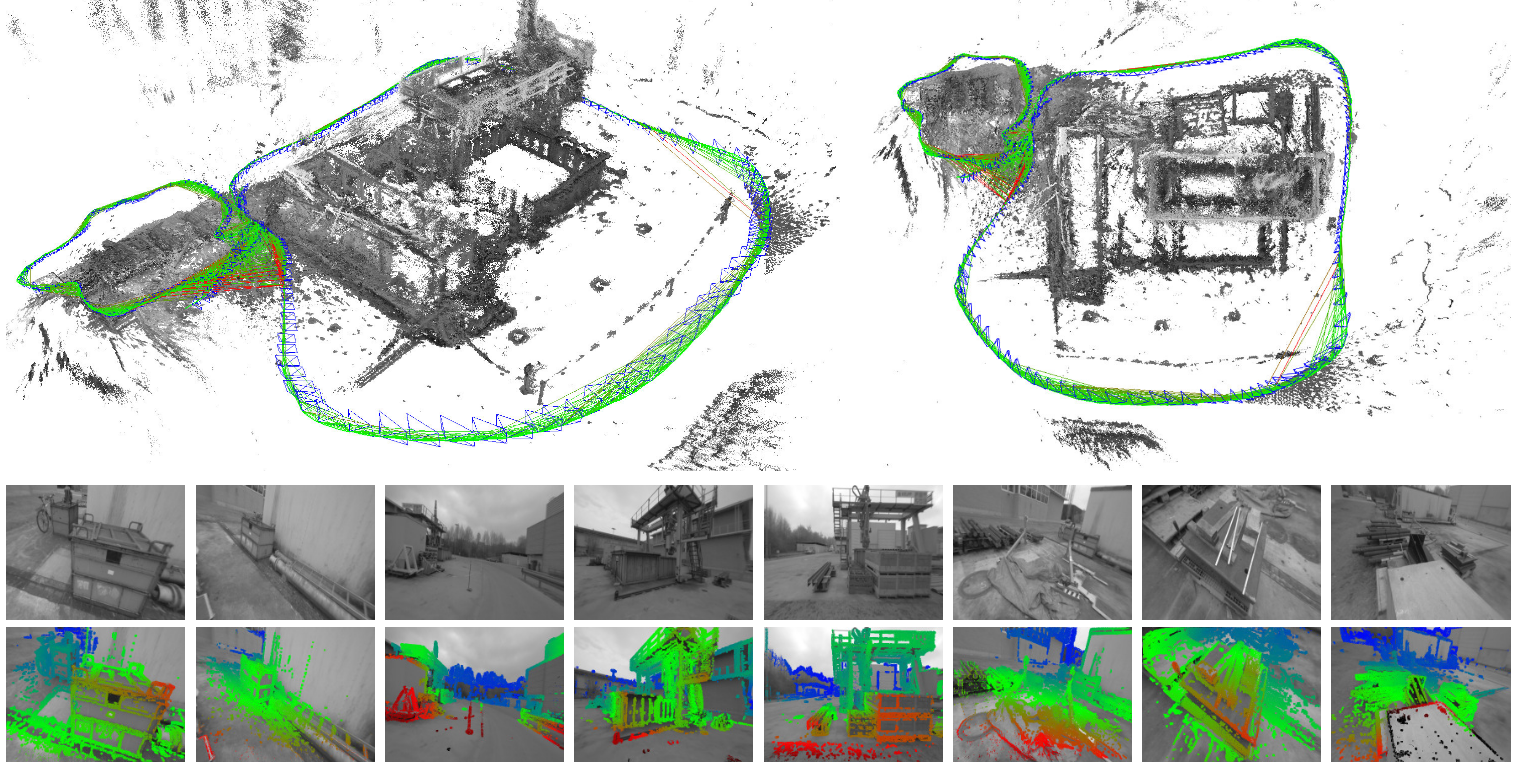
\includegraphics[height=0.5\textheight]{pics/lsd_slam_map_intro.png}
	\end{figure}

\end{frame}

%---------------------------------------
% Slide: Contribution
%---------------------------------------
\begin{frame}{\textcolor{blue}{\textbf{Contribution}}}
	\vspace{-0.5cm}
	\begin{itemize}
			\item Scale aware image alignment to estimate similarity transform $\boldsymbol{\xi} \in \mathfrak{s i m}(3)$ between two keyframes.
			\item Incorporation of depth uncertainty into tracking
	\end{itemize}

\end{frame}


%%%%%%%%%%%%%%%%%%%%%%%%%%%%%%%%%%%%%%%%
% Sub-section: Methodology
%%%%%%%%%%%%%%%%%%%%%%%%%%%%%%%%%%%%%%%%
\section*{\textbf{\textcolor{orange}{Methodology}}}
		\begin{frame}[plain]
				\vfill
			\centering
			\begin{beamercolorbox}[sep=8pt,center,shadow=true,rounded=true]{title}
				\usebeamerfont{title}\insertsectionhead\par%
				\color{oxfordblue}\noindent\rule{10cm}{1pt}
			\end{beamercolorbox}
			\vfill
	\end{frame}


%---------------------------------------
% Slide: Gauss Newton on Lie Manifolds
%---------------------------------------
\begin{frame}{\textcolor{blue}{\textbf{Gauss Newton on Lie Manifolds}}}
	\vspace{-0.5cm}
	\begin{block}{\textbf{\textcolor{teal}{3D Rigid Body Transformations}}}
	\begin{itemize}
			% G belongs to se(3) in latex
			\item 3D rigid body transform $G \in {SE}(3)$
			$$
				\mathbf{G}=\left(\begin{array}{cc}
				\mathbf{R} & \mathbf{t} \\
				\mathbf{0} & 1
				\end{array}\right) \quad \text { with } \quad \mathbf{R} \in \mathrm{SO}(3) \text { and } \mathbf{t} \in \mathbb{R}^3
			$$
			\item Optimization of camera pose is done on Lie algebra $\boldsymbol{\xi} \in \mathfrak{s i m}(3)$
			\item Mapping between Lie algebra and Lie group is given by:
			$$
				G = exp_{\mathfrak{se}(3)}(\boldsymbol{\xi}) \text{ and } \boldsymbol{\xi} = log_{\mathfrak{se}(3)}(G)
			$$
			\item Pose concatenation operator in Lie Algebra, $\circ : \mathfrak{s e}(3) \times \mathfrak{s e}(3) \rightarrow \mathfrak{s e}(3)$: 
			$$
				\boldsymbol{\xi}_{k i}:=\boldsymbol{\xi}_{k j} \circ \boldsymbol{\xi}_{j i}:=\log _{\mathrm{SE}(3)}\left(\operatorname{exp}_{\mathfrak{s e}(3)}\left(\boldsymbol{\xi}_{k j}\right) \cdot \operatorname{exp}_{\mathfrak{se}(3)}\left(\boldsymbol{\xi}_{j i}\right)\right)
			$$

	\end{itemize}

	\end{block}

\end{frame}


%---------------------------------------
% Slide: Gauss Newton on Lie Manifolds
%---------------------------------------
\begin{frame}{\textcolor{blue}{\textbf{Gauss Newton on Lie Manifolds}}}
	\vspace{-0.5cm}
	\begin{block}{\textbf{\textcolor{teal}{}}}
	\begin{itemize}
			\item Gauss Newton minimization of the photometric error
			\begin{equation}
				E(\boldsymbol{\xi})=\sum_i \underbrace{\left(I_{\mathrm{ref}}\left(\mathbf{p}_i\right)-I\left(\omega\left(\mathbf{p}_i, D_{\mathrm{ref}}\left(\mathbf{p}_i\right), \boldsymbol{\xi}\right)\right)\right)^2}_{=: r_i^2(\boldsymbol{\xi})},
			\end{equation}
			
			\begin{equation}
				\begin{aligned}
					\delta \boldsymbol{\xi}^{(n)}&=-\left(\mathbf{J}^T \mathbf{J}\right)^{-1} \mathbf{J}^T \mathbf{r}\left(\boldsymbol{\xi}^{(n)}\right)\\
					\boldsymbol{\xi}^{(n+1)}&=\delta \boldsymbol{\xi}^{(n)} \circ \boldsymbol{\xi}^{(n)}
				\end{aligned}
			\end{equation}

	\end{itemize}

	\end{block}

\end{frame}

	%---------------------------------------
% Slide: Algorithm Overview
%---------------------------------------
\begin{frame}{\textcolor{blue}{\textbf{Algorithm Overview}}}
	\vspace{-0.5cm}
	\begin{figure}
		\centering
		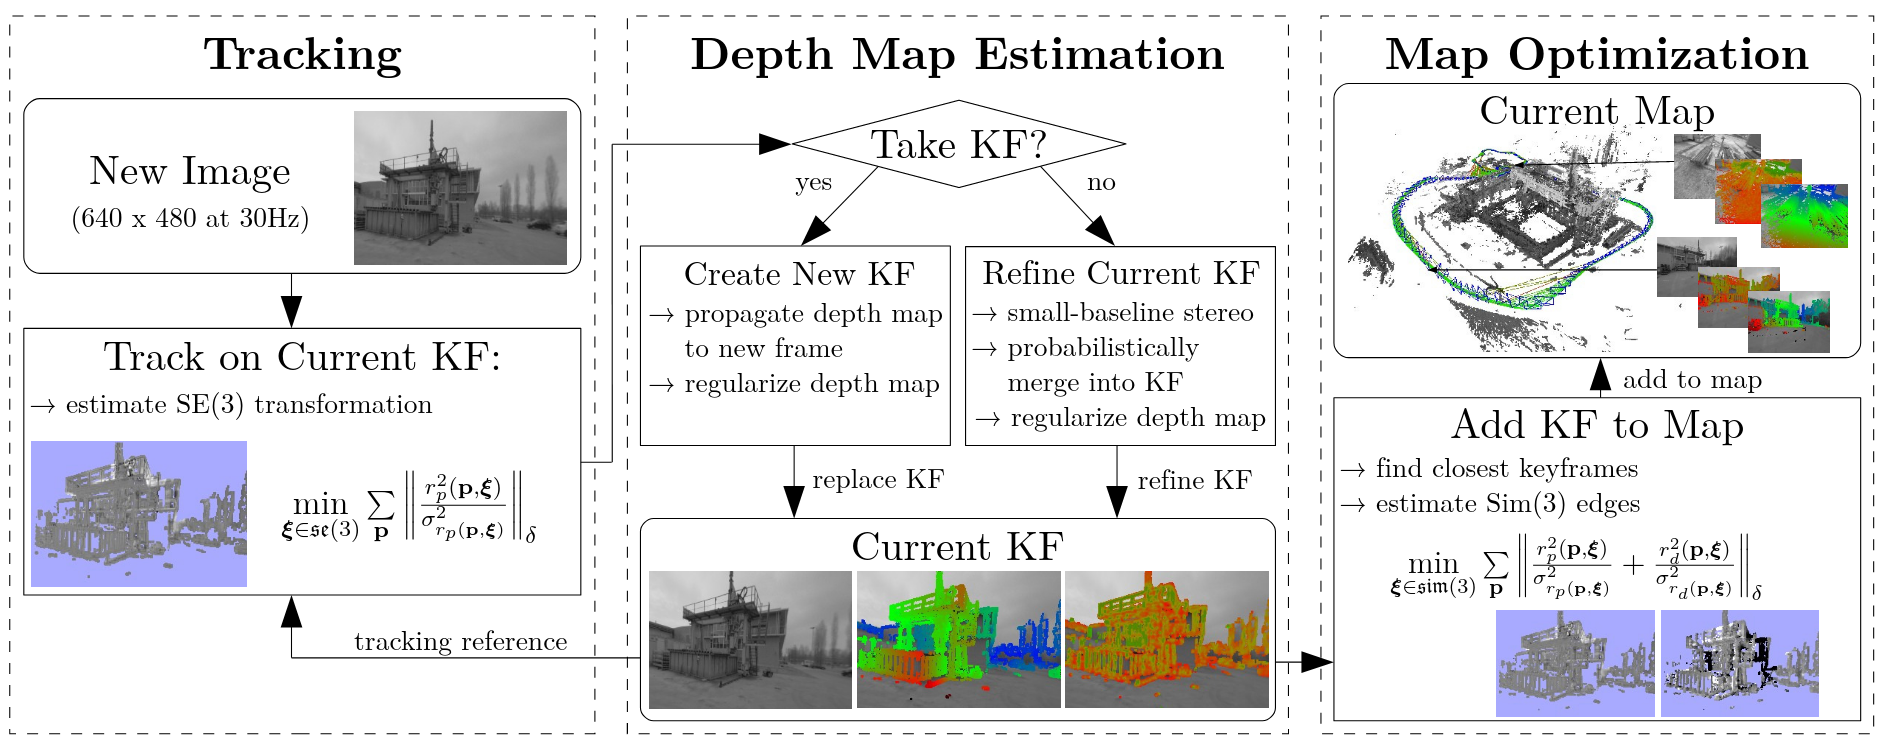
\includegraphics[height=0.6\textheight]{pics/algorithm_lsd_slam.png}
	\end{figure}
\end{frame}


%---------------------------------------
% Slide: Algorithm Overview
%---------------------------------------
\begin{frame}{\textcolor{blue}{\textbf{Algorithm Overview}}}
	\vspace{-0.5cm}
	% \begin{block}{\textbf{\textcolor{teal}{Statistics}}}
	\begin{itemize}
			\item \textbf{Depth Initialization} is done using indirect approach feature matching and stereo triangulation
			\item \textbf{Tracking} is done over new image and estimates $\boldsymbol{\xi} \in \mathfrak{s e}(3)$ with current Keyframe
			\item \textbf{Depth map refinement} is done by filtering at each pixel over small baseline stereo comparison
			\item \textbf{New Keyframe} is added if camera has moved more than a threshold
			\item \textbf{Map Optimization} is done over keyframes which are not currently track. Scale aware Loop closure, $\boldsymbol{\xi} \in \mathfrak{sim}(3)$ is incorporated in pose graph Optimization. 
	\end{itemize}

	% \end{block}

\end{frame}

%---------------------------------------
% Slide: Results
%---------------------------------------

\begin{frame}{\textcolor{blue}{\textbf{Results}}}
	\vspace{-0.8cm}
\begin{figure}
	\centering
	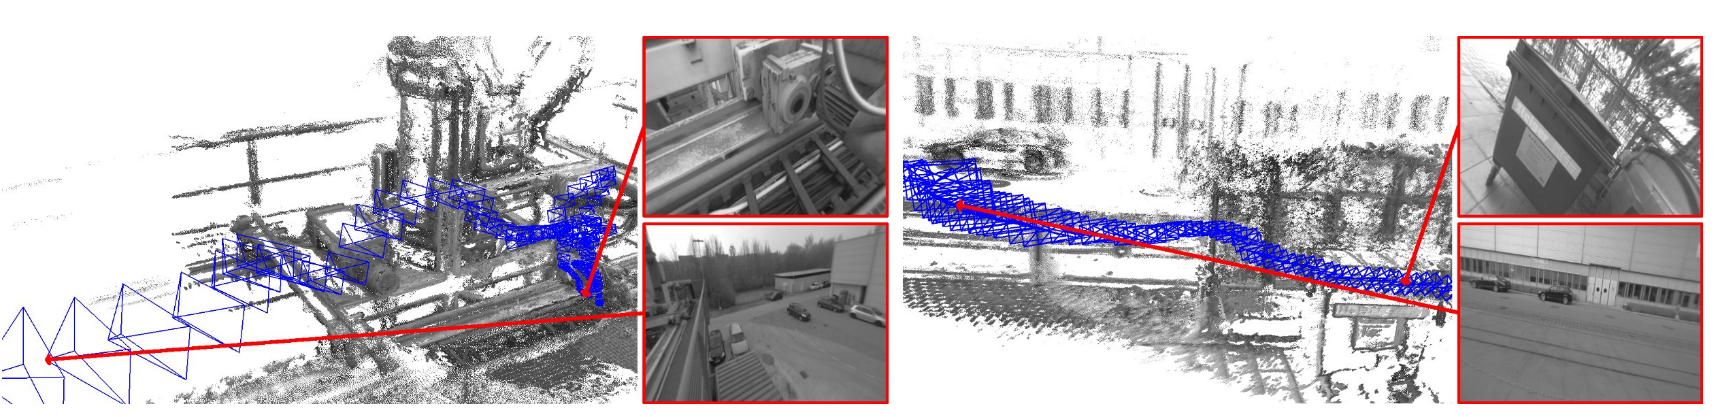
\includegraphics[width=0.7\textwidth]{pics/scale_drift_lsd_slam.png}
	\caption{Scale drift before map Optimization}
\end{figure}

\vspace{-0.8cm}

\begin{figure}
	\centering
	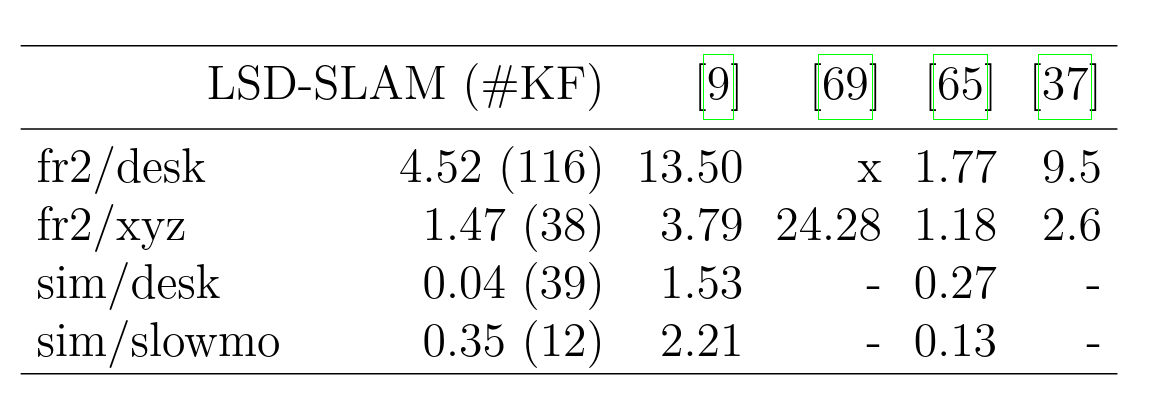
\includegraphics[width=0.7\textwidth]{pics/rmse_lsd.png}
	\caption{RMSE of estimated trajectory on TUM}
\end{figure}
\end{frame}

%---------------------------------------
% Slide: Results
%---------------------------------------

\begin{frame}{\textcolor{blue}{\textbf{Results}}}
	\vspace{-0.8cm}
\begin{figure}
	\centering
	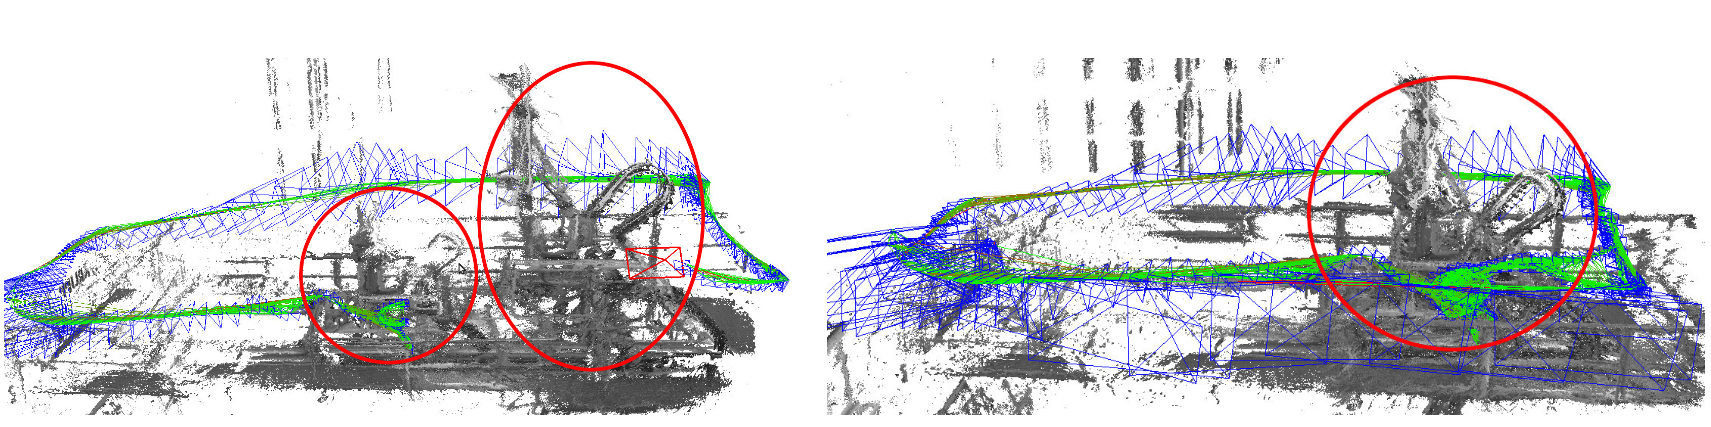
\includegraphics[width=0.95\textwidth]{pics/loop_closure_lsd.png}
	\caption{Average inverse depth varies from 20 cm to 10 m before loop closure and after loop closure geometry is consistently aligned}
\end{figure}

\end{frame}


%%%%%%%%%%%%%%%%%%%%%%%%%%%%%%%%%%%%%%%%
% Section: DSO  
%%%%%%%%%%%%%%%%%%%%%%%%%%%%%%%%%%%%%%%%
\section{\textbf{\textcolor{purple}{DSO : Direct Sparse Odometry}}}
		\begin{frame}[plain]
				\vfill
			\centering
			\begin{beamercolorbox}[sep=8pt,center,shadow=true,rounded=true]{title}
				\usebeamerfont{title}\insertsectionhead\par%
				\color{oxfordblue}\noindent\rule{10cm}{1pt}
			\end{beamercolorbox}
			\vfill

	\end{frame}

%---------------------------------------
% Slide: Introduction
%---------------------------------------
\begin{frame}{\textcolor{blue}{\textbf{Introduction}}}
	\vspace{-0.5cm}
	\begin{block}{\textbf{\textcolor{teal}{}}}
	\begin{itemize}
			\item Joint photometric error optimization over all model parameters
			\item Evenly sampling pixels in image space and avoiding smoothness prior
			\item Modelling full photometric calibration including vignetting, exposure time 
		\end{itemize}
	\end{block}

	\vspace{-0.4cm}

	\begin{figure}
		\centering
		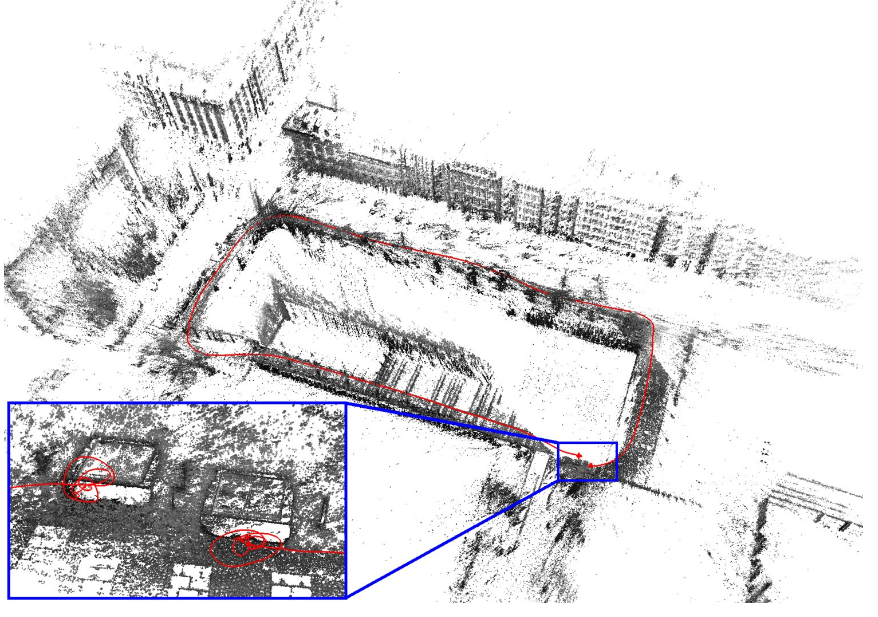
\includegraphics[height=0.5\textheight]{pics/dso_intro.png}
	\end{figure}

\end{frame}


%---------------------------------------
% Slide: Contribution
%---------------------------------------
\begin{frame}{\textcolor{blue}{\textbf{Contribution}}}
	\vspace{-0.5cm}
	\begin{block}{\textbf{\textcolor{teal}{}}}
	\begin{itemize}
			\item \textbf{Direct} samples pixels in weak intensity variation and sparse texture environments
			\item \textbf{Sparse} avoids smoothness and connectedness prior and runs in real-time
		\end{itemize}
	\end{block}

	\vspace{-0.4cm}

	\begin{figure}
		\centering
		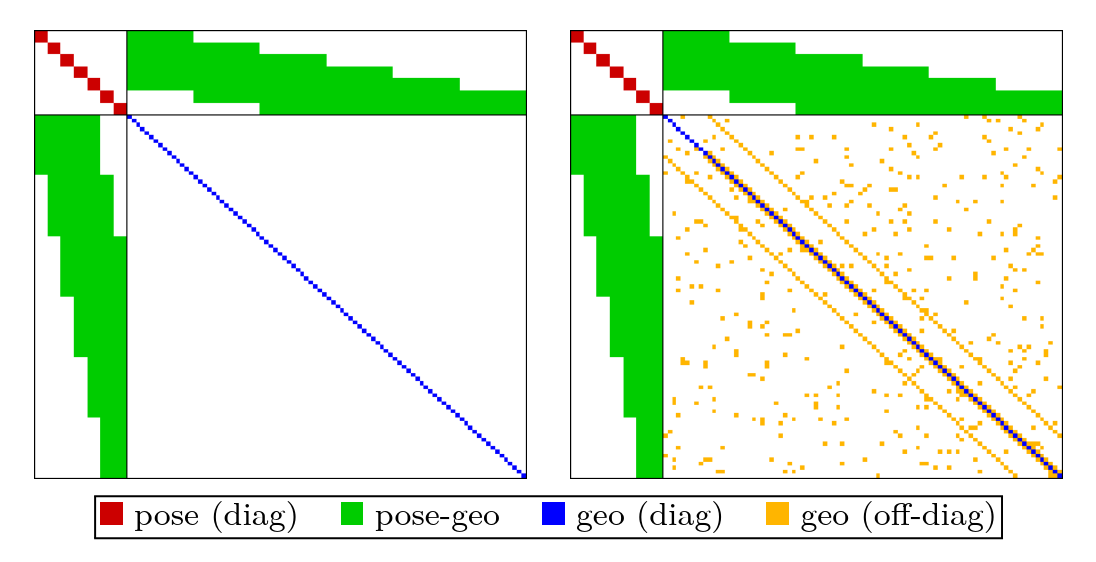
\includegraphics[height=0.5\textheight]{pics/hessian_matrix_sparsity.png}
	\end{figure}

\end{frame}

%---------------------------------------
% Slide: Schur Complement
%---------------------------------------
\begin{frame}{\textcolor{blue}{\textbf{Schur Complement}}}
	\vspace{-0.5cm}

	\begin{itemize}
			\item $\mathbf{H} \mathbf{x} = \mathbf{b}$ is expensive step in Gauss Newton Optimization
			\item When $x = \left[x_1, x_2\right]^T$ contains conditionally independent variables, we can solve the system in two steps
	\end{itemize}

	\begin{equation}
		\left(\begin{array}{ll}
		\mathbf{H}_{11} & \mathbf{H}_{12} \\
		\mathbf{H}_{21} & \mathbf{H}_{22}
		\end{array}\right)\left(\begin{array}{l}
		\mathbf{x}_1 \\
		\mathbf{x}_2
		\end{array}\right)=\left(\begin{array}{l}
		\mathbf{b}_1 \\
		\mathbf{b}_2
		\end{array}\right)
	\end{equation}

	\begin{equation}
		\begin{aligned}
			\left(\mathbf{H}_{11}-\mathbf{H}_{12} \mathbf{H}_{22}^{-1} \mathbf{H}_{21}\right) \mathbf{x}_1&=\left(\mathbf{b}_1-\mathbf{H}_{12} \mathbf{H}_{22}^{-1} \mathbf{b}_2\right)\\
			\mathbf{H}_{21} \mathbf{x}_1 + \mathbf{H}_{22} \mathbf{x}_2&=\mathbf{b}_2
		\end{aligned}
	\end{equation}

\end{frame}

%---------------------------------------
% Slide: Camera Calibration
%---------------------------------------
\begin{frame}{\textcolor{blue}{\textbf{Camera Calibration}}}
	\vspace{-0.5cm}
	
	\begin{block}{\textbf{\textcolor{teal}{Geometric Calibration}}}
	\begin{itemize}
			\item Pinhole camera model is used and radial distortion is removed
			\item Projection is $\Pi_{\mathbf{c}}: \mathbb{R}^3 \rightarrow \Omega$ and back projection is $\Pi_{\mathbf{c}}^{-1}: \Omega \times \mathbb{R} \rightarrow \mathbb{R}^3$
	\end{itemize}
	\end{block}

	\begin{block}{\textbf{\textcolor{teal}{Photometric Calibration}}}
	\begin{itemize}
			\item Surface irradiance $B_i$ defines radiant energy falling per unit area per unit solid angle
			\item Non-Linear response function $G$, exposure time $t_i$ and lens vignetting $V$ are used
			\begin{equation}
				\begin{aligned}
					I_i(\mathbf{x})&=G\left(t_i V(\mathbf{x}) B_i(\mathbf{x})\right)\\
					I_i^{\prime}(\mathbf{x})&:=t_i B_i(\mathbf{x})=\frac{G^{-1}\left(I_i(\mathbf{x})\right)}{V(\mathbf{x})}
				\end{aligned}
			\end{equation}
	\end{itemize}
	\end{block}

\end{frame}

%---------------------------------------
% Slide: Model Formulation
%---------------------------------------
\begin{frame}{\textcolor{blue}{\textbf{Model Formulation}}}
	\vspace{-0.5cm}
	\begin{itemize}
			\item Photometric error of point $\mathbf{p} \in \Omega_i$ observed in frame in $I_j$, is $E_{\mathbf{p}j}$
			\item Weighted sum of squared differences is done over 8 pixels in a 3x3 window
			\begin{equation}
				E_{\mathbf{p} j}:=\sum_{\mathbf{p} \in \mathcal{N}_{\mathbf{p}}} w_{\mathbf{p}}\left\|\left(I_j\left[\mathbf{p}^{\prime}\right]-b_j\right)-\frac{t_j e^{a_j}}{t_i e^{a_i}}\left(I_i[\mathbf{p}]-b_i\right)\right\|_\gamma
			\end{equation}
	\end{itemize}

	\begin{equation}
		\begin{aligned}
		&\mathbf{p}^{\prime}=\Pi_{\mathbf{c}}\left(\mathbf{R} \Pi_{\mathbf{c}}^{-1}\left(\mathbf{p}, d_{\mathbf{p}}\right)+\mathbf{t}\right)\\
		&\left[\begin{array}{cc}
		\mathbf{R} & \mathbf{t} \\
		0 & 1
		\end{array}\right]:=\mathbf{T}_{i}^{j}
		\end{aligned}
	\end{equation}

	\begin{figure}
		\centering
		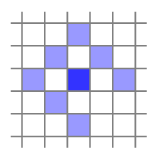
\includegraphics[height=0.2\textheight]{pics/residual_pattern.png}
	\end{figure}

\end{frame}


%---------------------------------------
% Slide: Model Formulation
%---------------------------------------
\begin{frame}{\textcolor{blue}{\textbf{Model Formulation}}}
	\vspace{-0.5cm}
	\begin{itemize}
			\item Geometric and photometric variables $\left[T_i, T_j , d, c, a_i, a_j , b_i, b_j\right]$ are optimized jointly
			\item Full photometric error over all frames $\mathcal{F}$, over all points $\mathcal{P}_i$ in frame $i$:
			
			\begin{equation}
				E_{\text {photo }}:=\sum_{i \in \mathcal{F}} \sum_{\mathbf{p} \in \mathcal{P}_i} \sum_{j \in \mathrm{obs}(\mathbf{p})} E_{\mathbf{p} j} 
			\end{equation}
	\end{itemize}

	\vspace{-0.5cm}

	\begin{figure}
		\centering
		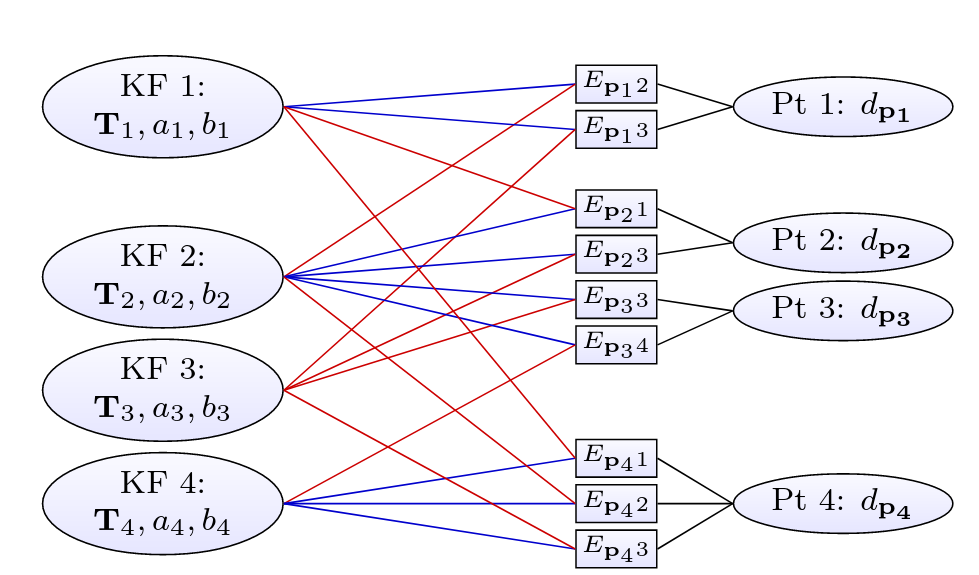
\includegraphics[height=0.4\textheight]{pics/dso_factor_graph.png}
	\end{figure}

\end{frame}


%---------------------------------------
% Slide: Windowed Optimization
%---------------------------------------
\begin{frame}{\textcolor{blue}{\textbf{Windowed Optimization}}}
	\vspace{-0.5cm}
	\begin{itemize}
			\item All variables are denoted $\zeta \in SE(3)^n \times \mathbb{R}^m$ and its Lie Algebra $x \in \mathfrak{se}(3)^n \times \mathbb{R}^m$
			\item Single residual $r_k$ and its Jacobian $J_k$ are:
	\end{itemize}

	\begin{equation}
		\begin{aligned}
		r_k & =r_k\left(\boldsymbol{x} \boxplus \boldsymbol{\zeta}_0\right) \\
		& =\left(I_j\left[\mathbf{p}^{\prime}\left(\mathbf{T}_i, \mathbf{T}_j, d, \mathbf{c}\right)\right]-b_j\right)-\frac{t_j e^{a_j}}{t_i e^{a_i}}\left(I_i[\mathbf{p}]-b_i\right)
		\end{aligned}
	\end{equation}

	\begin{equation}
			\mathbf{J}_k=[\underbrace{\frac{\partial I_j}{\partial \mathbf{p}^{\prime}}}_{\mathbf{J}_I} \underbrace{\frac{\partial \mathbf{p}^{\prime}\left((\boldsymbol{\delta}+\boldsymbol{x}) \boxplus \boldsymbol{\zeta}_0\right)}{\partial \boldsymbol{\delta}_{\text {geo }}}}_{\mathbf{J}_{\text {geo }}}, \underbrace{\frac{\partial r_k\left((\boldsymbol{\delta}+\boldsymbol{x}) \boxplus \boldsymbol{\zeta}_0\right)}{\partial \boldsymbol{\delta}_{\text {photo }}}}_{\mathbf{J}_{\text {photo }}}]
	\end{equation}

	\begin{itemize}
			\item Update is $x^{new} \leftarrow \delta + x$
	\end{itemize}

\end{frame}


%%%%%%%%%%%%%%%%%%%%%%%%%%%%%%%%%%%%%%%%
% Sub-section: Visual Odometry Frontend
%%%%%%%%%%%%%%%%%%%%%%%%%%%%%%%%%%%%%%%%
\section*{\textbf{\textcolor{orange}{Visual Odometry Frontend}}}
		\begin{frame}[plain]
				\vfill
			\centering
			\begin{beamercolorbox}[sep=8pt,center,shadow=true,rounded=true]{title}
				\usebeamerfont{title}\insertsectionhead\par%
				\color{oxfordblue}\noindent\rule{10cm}{1pt}
			\end{beamercolorbox}
			\vfill
	\end{frame}


%---------------------------------------
% Slide: Frame Management
%---------------------------------------
\begin{frame}{\textcolor{blue}{\textbf{Frame Management}}}
	\vspace{-0.5cm}
	\begin{itemize}
			\item \textbf{Initial Frame Tracking} is done using \textit{direct image alignment} over \textit{multi-scale image pyramid}
			\item \textbf{Keyframe Creation} is done when mean square  optical flow $f:=\left(\frac{1}{n} \sum_{i=1}^n\left\|\mathbf{p}-\mathbf{p}^{\prime}\right\|^2\right)^{\frac{1}{2}}$ greater than threshold
			\item \textbf{Keyframe Creation} is done when camera translation causes occlusion or if the camera exposure changes 
	\end{itemize}

\end{frame}


%---------------------------------------
% Slide: Frame Management
%---------------------------------------
\begin{frame}{\textcolor{blue}{\textbf{Frame Management}}}
	\vspace{-0.5cm}
	\begin{block}{\textbf{\textcolor{teal}{Keyframe marginalization}}}
	\begin{itemize}
			\item Active keyframes: $\left[I_1, ..., I_n\right]$, with $I_1$ is latest and $I_n$ is oldest
			\item Frames with less than $5\%$ points visible in $I_1$ are marginalized
			\item Frames which maximizes distance score $s(I_i)$ are marginalized
	\end{itemize}
	\end{block}

	\begin{equation}
		s\left(I_i\right)=\sqrt{d(i, 1)} \sum_{j \in[3, n] \backslash\{i\}}(d(i, j)+\epsilon)^{-1}
	\end{equation}

\end{frame}


%---------------------------------------
% Slide: Frame Management
%---------------------------------------
\begin{frame}{\textcolor{blue}{\textbf{Frame Management}}}
	\vspace{-1cm}

	\begin{figure}
		\centering
		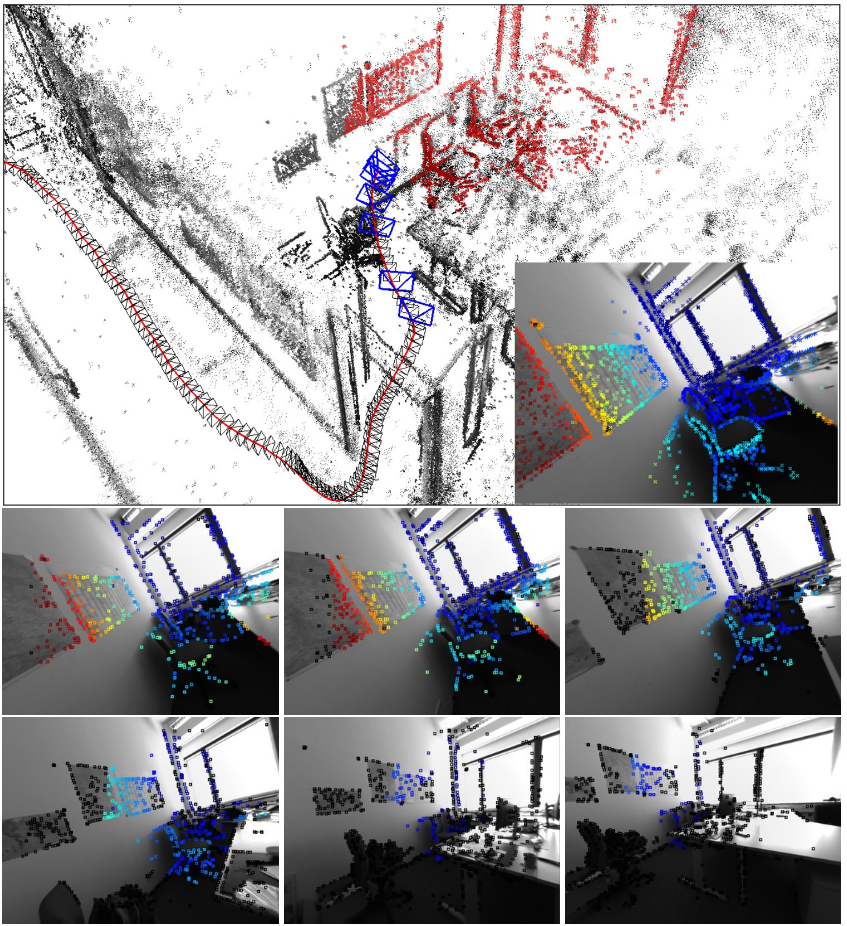
\includegraphics[height=0.6\textheight]{pics/keyframe_marginal_dso.png}
		\caption{
			Bottom row: 6 old keyframes with points overlaid, black points are already marginal.
			Top row: All active and past camera positions, active points and keyframes are shown in red and blue respectively.
		}
	\end{figure}

\end{frame}




%---------------------------------------
% Slide: Point Management
%---------------------------------------
\begin{frame}{\textcolor{blue}{\textbf{Point Management}}}
	\vspace{-0.5cm}
	\begin{itemize}
			\item Fix number of $N_P = 2000$ points are active across space and frames for optimization
			\item \textbf{Candidate Point Selection} is done by splitting image into $d \times d$ blocks and largest gradient point is selected 
			\item \textbf{Candidate Point Tracking} are track along epipolar lines by minimizing photometric error
			\item \textbf{Candidate Point Activation} is done by projecting points into current keyframe and maximizing distance to previous points
	\end{itemize}

\end{frame}


%---------------------------------------
% Slide: Results
%---------------------------------------

\begin{frame}{\textcolor{blue}{\textbf{Results}}}
	\vspace{-0.8cm}

	\begin{itemize}
		\item Evaluation done on TUM monoVO, EuRoC MAV and ICL-NUIM datasets
	\end{itemize}

	\begin{figure}
		\centering
		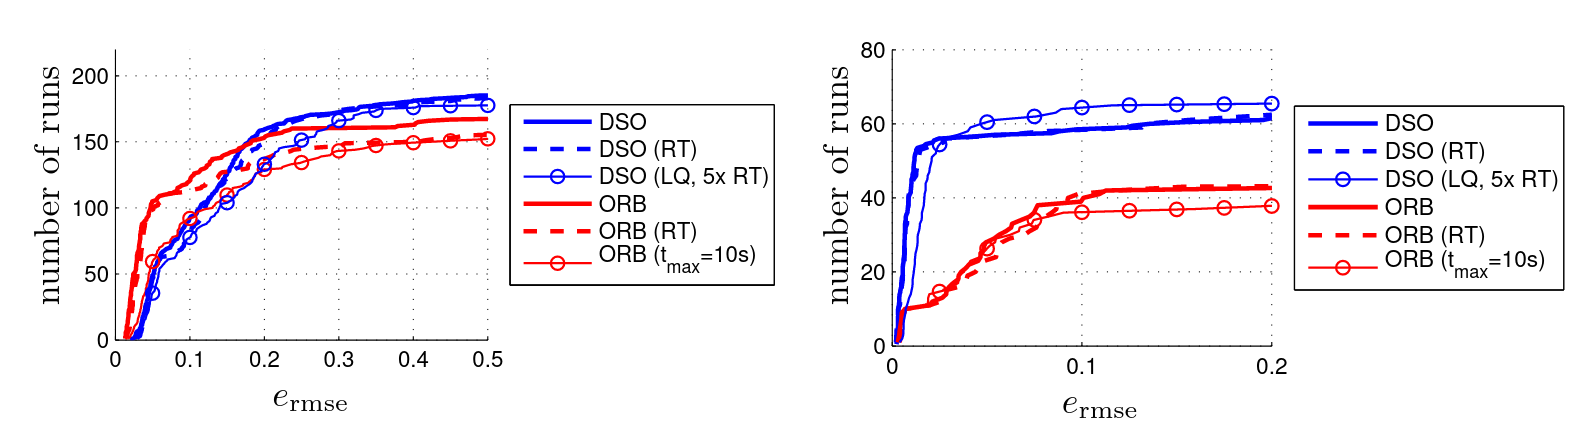
\includegraphics[width=0.8\textwidth]{pics/eruoc_mav_and_icl.png}
		\caption{EuRoC MAV and ICL-NUIM RMSE Error}
	\end{figure}
\end{frame}


\begin{frame}{\textcolor{blue}{\textbf{Results}}}
	\vspace{-1cm}

	\begin{figure}
		\centering
		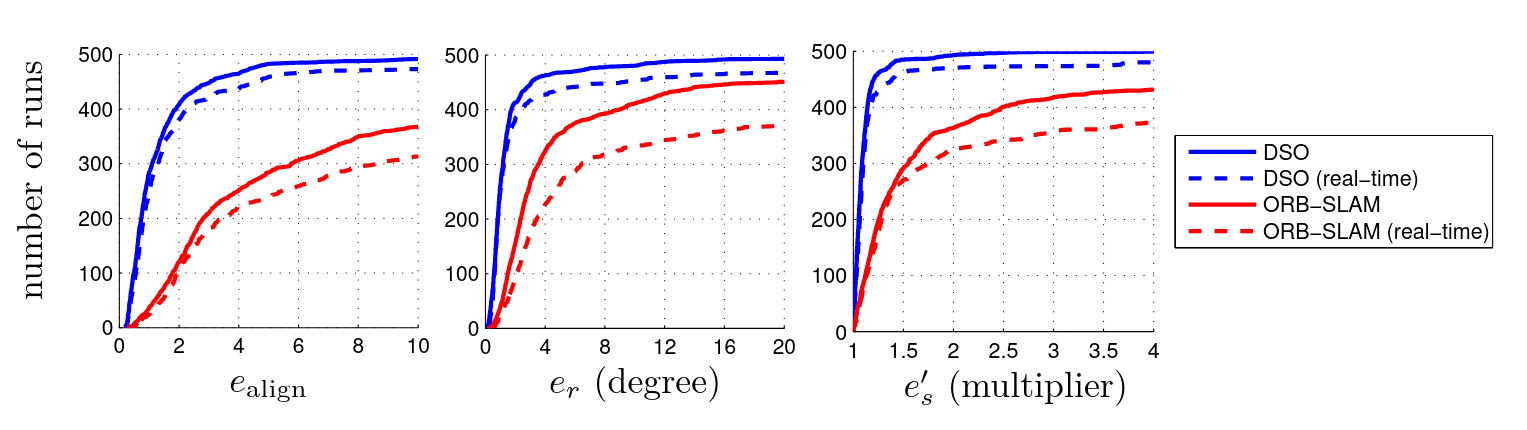
\includegraphics[width=0.5\textwidth]{pics/tum_mono.png}
		\caption{Accumulated Rotation and scaling drift after large a loop}
	\end{figure}

	\vspace{-1cm}

	\begin{figure}
		\centering
		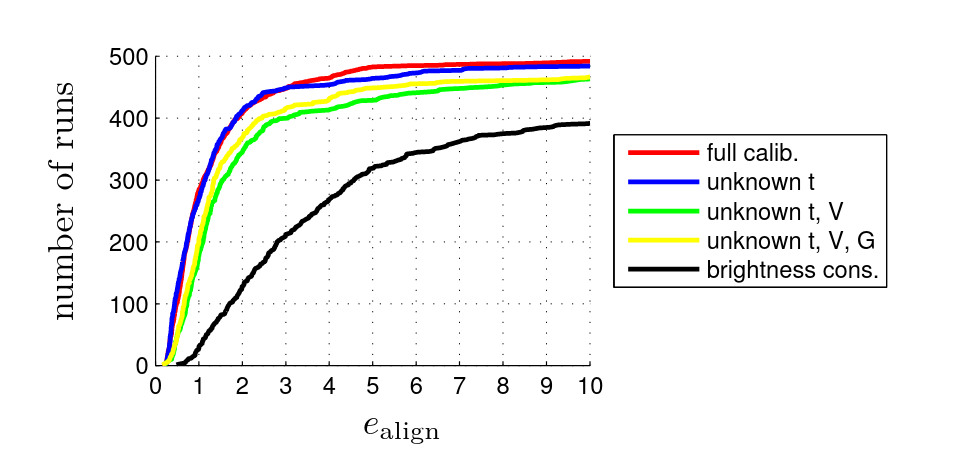
\includegraphics[width=0.5\textwidth]{pics/photometric_params.png}
		\caption{From fully photometric calibration to no photometric calibration effect on TUM-monoVO Dataset}
	\end{figure}

\end{frame}

%%%%%%%%%%%%%%%%%%%%%%%%%%%%%%%%%%%%%%%%
% Section: Limitations and Future Work  
%%%%%%%%%%%%%%%%%%%%%%%%%%%%%%%%%%%%%%%%
\section{\textbf{\textcolor{purple}{Limitations and Future Work}}}
		\begin{frame}[plain]
				\vfill
			\centering
			\begin{beamercolorbox}[sep=8pt,center,shadow=true,rounded=true]{title}
				\usebeamerfont{title}\insertsectionhead\par%
				\color{oxfordblue}\noindent\rule{10cm}{1pt}
			\end{beamercolorbox}
			\vfill

		\begin{itemize}
				\item High non-linearity in photometric error causes optimization to be strong non-convex
				\item Need for accurate initialization: Pose can be initialized using IMU
				\item Depth is initialized using search along epipolar line: Depth can be initialized using Monocular Depth Network
				\item Indirect approaches are more robust in detection and relocation of loop closures in illumination and viewpoint changes
				\item Zeroth-order information of absolute intensity is used: Residual can incorporate first and second order information
		\end{itemize}
	\end{frame}


\begin{frame}{\textcolor{blue}{\textbf{References}}}
	\vspace{-0.5cm}
	\begin{itemize}
			\item Direct Sparse Odometry
			\item Large-Scale Direct Monocular SLAM
	\end{itemize}
\end{frame}

%%%%%%%%%%%%%%%%%%%%%%%%%%%%%%%%%%%%%%%%
% Slide: Last Slide 
%%%%%%%%%%%%%%%%%%%%%%%%%%%%%%%%%%%%%%%%
\begin{frame}{}
		\begin{center}

				% Writing above poem in latex
				% \textbf{\textcolor{blue!70}{\large ``Direct Sparse Odometry, a marvel to behold}}\\
				% \textbf{\textcolor{blue!70}{\large Photometric camera alignment, a story to be told,}}\\
				% \textbf{\textcolor{blue!70}{\large Gauss-Newton optimization, a powerful tool,}}\\
				% \textbf{\textcolor{blue!70}{\large Together they create a mapping wonder, a true jewel"}}\\

				\vspace{10mm}
				\textbf{\textcolor{teal!80}{\huge  Thank You!}}
		\end{center}
\end{frame}

\end{document}
